% ===================================================
% CHAPITRE 17 — LA GRANDE RÉVOLUTION
% Pages imprimées 141-166 — vues 144-169
% ===================================================
\chapter{La Grande Révolution}

% --- Page imprimée 141 — vue 144
REVOLUTION

\begin{figure}[ht]
    \centering
    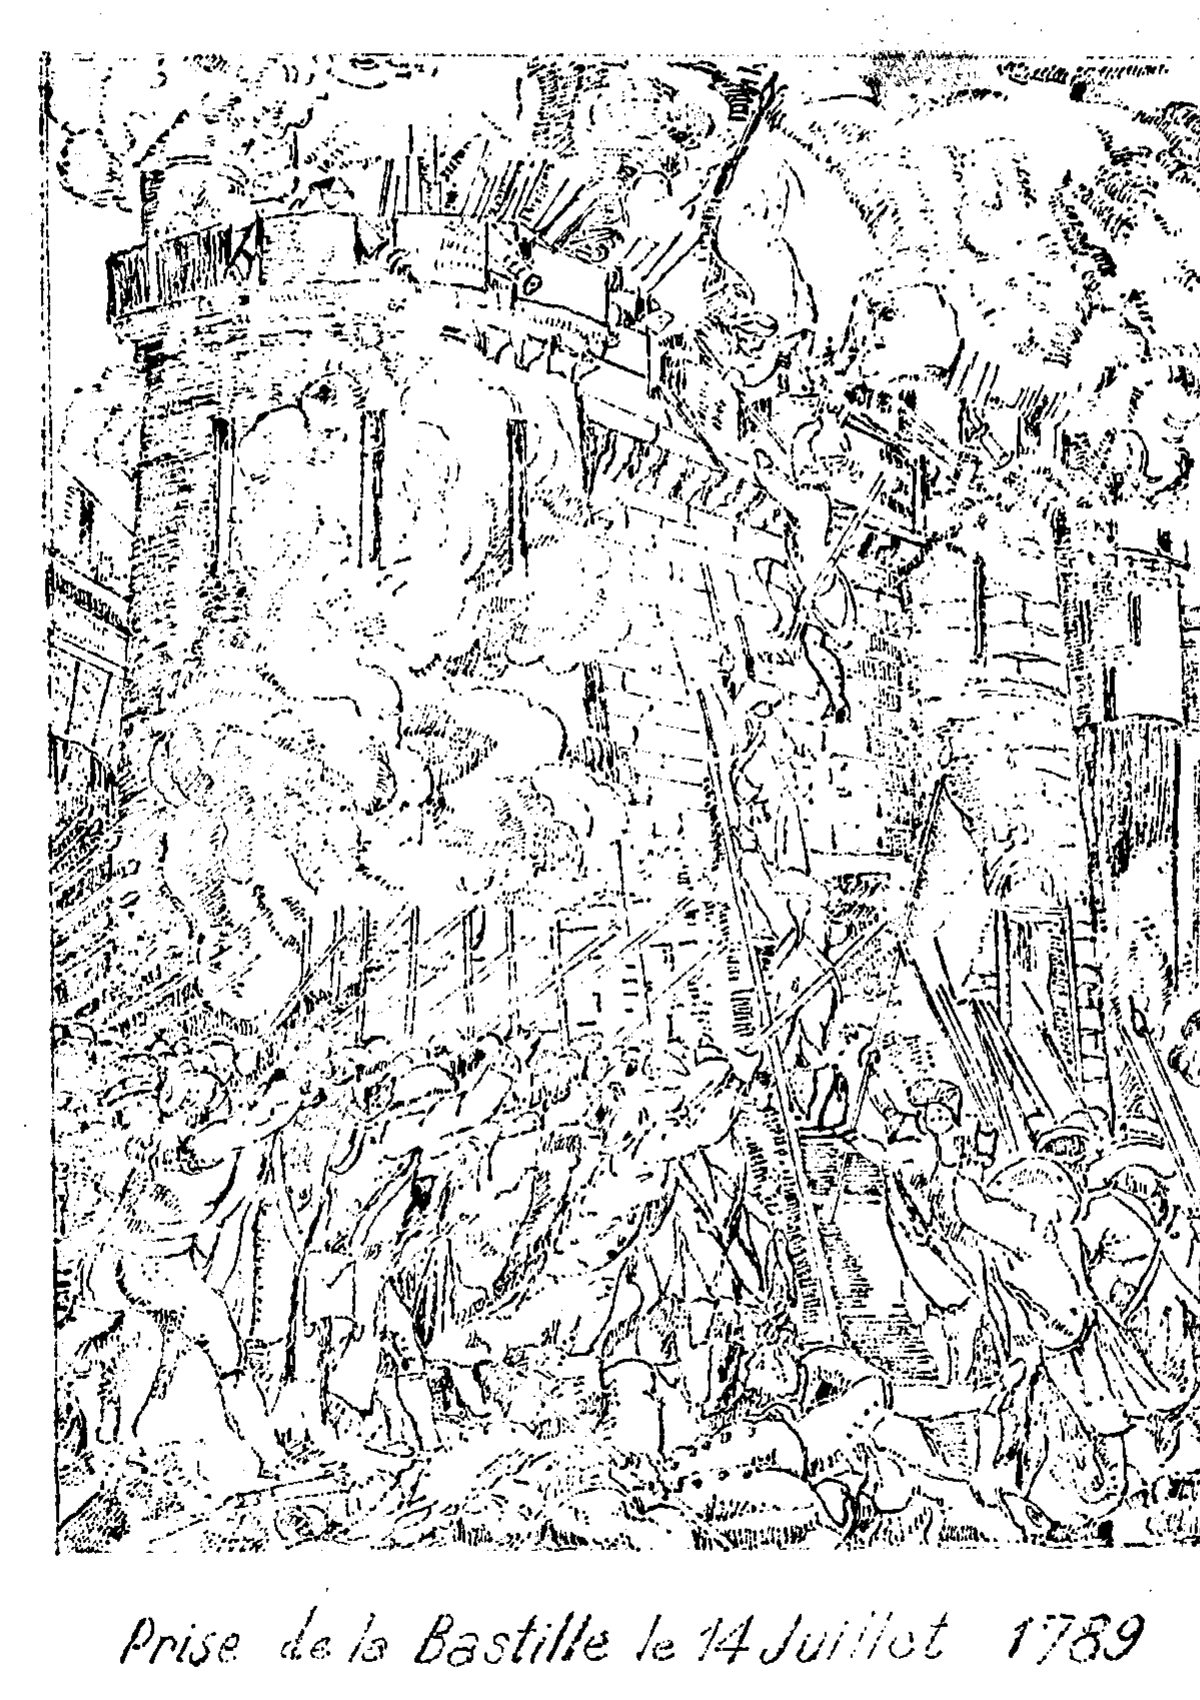
\includegraphics[width=0.48\textwidth]{Illustrations/illus-revolution-bastille.png}
\end{figure}

% --- Page imprimée 142 — vue 145
L'histoire d'Ouroux durant la période révolutionnaire offrirait à cette heure un intérêt exceptionnel ; malheureusement aucun des témoins des nombreux épisodes dont notre contrée fut le théâtre n'a eu la pensée de laisser à la postérité un récit détaillé de ce qu'il avait vu ou entendu. Le souvenir des anciens qui vivent encore est tellement confus, tellement vague qu'il ne peut être d'aucun secours dans les recherches. Néanmoins ce que nous avons pu recueillir suffira pour nous donner une idée assez complète de ce que fut notre paroisse pendant ces années de persécutions et de terreur.

Mr Morétain avouait lui-même n'avoir presque rien appris. Nous utiliserons, dans la mesure du possible, les quelques notes qu'il a laissées et les faits les plus saillants qu'il a pu nous transmettre. L'auteur de la France par Cantons, Mr Ogier, n'a fait que mettre en ordre le récit que lui avait fourni Mr Morétain.

Pour bien juger les évènements qui se déroulèrent parmi nous vers la fin du XVIIIème siècle, il est bon de nous demander quelle était en 1789 la situation de St-Antoine d'Ouroux.

Nous l'avons vu, Mr Guillin avait laissé cette paroisse dans une situation prospère. Mr Trouilloux avait dignement continué son œuvre. Depuis plus de vingt ans, comme vicaire ou comme curé, il se dévouait à l'éducation intellectuelle et morale de l'enfance et donnait une direction éclairée aux âmes qui lui avaient été confiées. Son influence était par conséquent considérable autour de lui.

Depuis un an d'ailleurs il se trouvait dignement secondé par Mr Odin, son vicaire, lorsque les mauvais jours arrivèrent.

Notre paroisse ne renfermait aucun de ces éléments de dissolutions que l'on trouve ailleurs à cette époque. Point de grandes propriétés, point de seigneurs et partant point de ces haines qu'une étincelle suffisait à attiser. Les six fiefs qui se trouvaient à

% --- Page imprimée 143 — vue 146
Ouroux ou sur ses limites n'offraient rien qui put exciter la cupidité des sectaires. Leurs possesseurs ne résidaient pas ; seuls les barons de Lacarelle passaient une partie de l'année dans leur château.

Nulle industrie, des voies de communications difficilement praticables, pas de centres importants dans le voisinage. Aussi les excitations venues du dehors purent-elles rester sans écho. Les membres des comités révolutionnaires eurent beau lancer leurs émissaires contre plusieurs châteaux du Beaujolais, ils s'arrêtèrent devant celui du Truil qu'ils brûlèrent, il est vrai, mais ils ne franchirent pas la montagne.

Notre vallée aurait pu craindre cependant de voir se renouveler les scènes sanglantes dont le Lyonnais et le Beaujolais furent si souvent le théâtre. Mr Antoine Guillin du Montet, seigneur de Pougelon, le Sauzay, Avenas, etc. était regardé, nous l'avons vu plus haut, comme le chef de la Contre-révolution dans nos contrées. La famille qui avait tout à redouter de la part des ennemis du roi, se retira au Sauzay. Personne néanmoins n'y fut inquiété jusqu'au jour où tous les membres de la famille émigrèrent.

Les Seigneurs de Lacarelle avaient eu, eux aussi, l'honneur de montrer leur dévouement à la cause royale.

Henri Jean de la Roche, baron de Montcel, seigneur de la Peyrouse et autres lieux, était né à St-Domingue le 10 Septembre 1753. Entré dans la 2ème compagnie des mousquetaires du roi en 1770, il avait été breveté Capitaine de cavalerie à la réforme de la garde royale, et reçu chevalier de l'ordre royal et militaire de St Louis par lettres patentes du 22 Aout 1814. Il s'offrit en 1791 comme otage pour sa Majesté Louis XVI après son retour de Varennes. Il fut reçu cette même année membre de l'ordre et archiconfrérie du St-Sépulcre de Jérusalem.

Son frère Jean-Marie de La Roche, chevalier, baron de La Roche, seigneur de Lacarelle et autres lieux, était né également à St-Domingue le 16 Octobre 1754. Entré comme son frère en 1770, à la 2ème compagnie des Mousquetaires du roi, il avait été nommé à la réforme du corps en 1776, officier au régiment du Cap français et avait fait
% --- Page imprimée 144 — vue 147 (suite)
en cette qualité les guerres d'Amérique. Il fut reçu chevalier de l'Ordre Royal et militaire de St-Louis par brevet du 30 Mai 1814. Il fit également partie des mille royalistes dévoués qui s'offrirent en otage pour Louis XVI et sa famille.

Néanmoins malgré leurs titres à la haine des ennemis de l'ordre, il ne paraît pas que les seigneurs de Lacarelle aient eu à souffrir à cette époque ; peut-être les concessions qu'ils crurent devoir faire au schisme leur épargnèrent-elles les haines des révolutionnaires

Les Seigneurs de la Barmondière possesseurs des fiefs d'Arcis et les Comtes de Fautrières seigneurs de Montolieu ne résidaient pas.

Les années qui précédèrent la tourmente révolutionnaire s'écoulèrent donc au milieu du calme le plus absolu. La tranquillité ne fut même pas troublée par cet instant de panique rapporté par tous les historiens et qui jeta la France entière dans l'effroi. On se rappelle que le même jour et à la même heure le bruit courait dans chaque paroisse qu'une armée de brigands approchait et mettait tout à feu et à sang. On sonnait le tocsin, les municipalités organisaient la défense, la garde nationale courait aux armes. Bientôt on constatait que ce n'était qu'une fausse alerte.

À Ouroux, grâce à la présence d'esprit de Mr le Curé Trouilloux, rien de semblable n'eut lieu. Sur ses conseils on s'abstint de sonner le tocsin. "Laissez faire, disait-il, il n'arrivera que ce que le Bon Dieu voudra". Peu de paroisses en France surent, au milieu de l'effervescence générale, conserver leur calme comme la nôtre.

Il fallait l'odieuse loi qui porte dans l'histoire le titre de Constitution civile du Clergé pour introduire parmi nous le désordre. Le clergé mis en demeure de choisir entre sa conscience et les prescriptions d'une loi impie n'hésita pas et l'immense majorité préféra affronter la persécution la plus inique plutôt que de rompre avec l'unité de l'Église.

Mr Trouilloux avait donné trop de preuves de son énergie et de son attachement à la vraie foi pour que l'on pût craindre un instant de le voir défaillir. Il refusa énergiquement de prêter le serment exigé par le gouvernement français et condamné à Rome par le Souverain Pontife : "Je jure de maintenir de tout mon pouvoir la liberté,
% --- Page imprimée 145 — vue 148 (suite)
l'égalité et de mourir s'il le fallait pour l'exécution de la loi".
Ce serment qui excita d'unanimes réprobations devait être remplacé, plus tard, par celui-ci : "Je reconnais que l'universalité des Français est le Souverain et je promets soumission et obéissance aux lois de la République". Par une Bulle du 5 Juillet 1796 le Pape toléra cette nouvelle formule.

Il y eut d'abord certaines hésitations relativement à la licéité du premier serment. Des prêtres distingués croyaient pouvoir l'interpréter dans un sens favorable. Mr Trouilloux prit pour guide de sa conduite le sentiment formellement exprimé par l'autorité diocésaine. Mr Odin se fit un devoir de suivre son exemple et refusa, lui aussi, le serment exigé.

Mr Trouilloux, en vertu de la loi perdait son titre de curé ; l'autorité gouvernementale avait donc à lui donner un successeur. Mais à cette époque les populations de nos campagnes que l'athéisme n'avait pas encore égarées, que les clubs ne pouvaient atteindre de leurs secrètes intrigues et de leurs discours impies et scandaleux, ces populations étaient fermement attachées à leurs prêtres. Et Ouroux qui avait su apprécier le dévouement et la sainteté de son vénéré pasteur ne pouvait laisser s'accomplir une pareille iniquité sans protester. Bien plus, il sut opposer la force ouverte aux empiétements du pouvoir illégitime ; mais surtout il offrit un exemple frappant de ce que peut une résistance passive mais persévérante en face de l'audace des impies.

Mr Trouilloux et Mr Odin quittèrent donc le presbytère de la paroisse pour faire place au curé intrus que les autorités du district de Villefranche venaient d'agréer. Cette nomination ne se fit sans doute pas sans quelque difficulté. La loi, en effet, avait été promulguée en Décembre 1790 ; nous ne trouvons néanmoins aucune trace du successeur avant le 11 Juillet 1791.

Il est inutile d'ajouter que nous n'avons sur les deux prêtres assermentés qui furent mis successivement à la tête de la paroisse, aucun renseignement. L'un ne nous est connu que par une seule signature ; l'autre, bien qu'ayant séjourné ici plus longtemps, n'a guère laissé plus de traces. Cette absence de renseignements s'ex
% --- Page imprimée 146 — vue 149 (suite)
plique du reste facilement. Le nombre des prêtres qui prêtèrent serment fut relativement peu considérable ; beaucoup reconnurent leur erreur et se rétractèrent. Généralement celui qui persistait dans le schisme ne pouvait guère conserver la direction de la paroisse qu'il avait précédemment administrée et alors il allait, au loin, offrir le secours de son ministère ou cacher son infamie. Nous ignorons donc absolument d'où venaient les deux intrus qui résidèrent quelque temps au milieu de nous et ce qu'ils devinrent après leur départ de la paroisse.

Il est bon d'observer aussi que les dates concernant la période révolutionnaire sont difficiles à débrouiller ; les registres de la fabrique ne sont plus tenus régulièrement ; les actes de l'état religieux sont eux-mêmes écrits après coup et pour la plupart au retour de Mr Trouilloux ; ils ne peuvent dès lors nous offrir que des probabilités.

Le premier qui prit possession de la cure fut un nommé Auberger, que Mr Morétain nomme simplement Berger mais à tort comme le prouve l'acte de Baptême de Antoine Louis Ferdinand fils de Jean Marie de La Roche de Lacarelle, au bas duquel nous trouvons sa signature.

Consciencieux observateur de la loi de Juin 1790 qui interdit l'usage des titres honorifiques et de toute qualification féodale il eut bien soin de supprimer dans l'acte le titre de baron et il fallut un jugement rendu par le tribunal de Villefranche le 16 Mars 1855 pour le rétablir. Le Baptême de cet enfant eut lieu le 11 Juillet 1791.

L'opposition déclarée de la population tout entière ne lui permit pas d'attendre les résultats d'un ministère condamné d'avance à l'impuissance. Il se découragea et partit. Son successeur nommé Barthélemy était installé le 8 Octobre 1791 jour où nous le voyons faire son premier enterrement.

Ce dernier, paraît-il, était membre de plusieurs académies ; c'est du moins ce qu'il affirme à la suite d'une de ses signatures.

Quelle était pendant ce temps là la situation de Mr le Curé Trouilloux et de Mr Odin ?

Auberger qui affrontait le premier des difficultés exceptionnelles fit valoir consciencieusement, sans doute, ses droits et n'entretint
% --- Page imprimée 147 — vue 150 (suite)
aucun rapport avec eux. Ceux-ci d'ailleurs durent trouver une maison hospitalière dans le bourg et ils pouvaient dire facilement la Sainte Messe dans les chapelles soit du château Guillin, soit du château de Grosbois ou de Lacarelle.

Mais Barthélemy, comprenant qu'il valait mieux user de douceur que de violence, voulut montrer quel était son esprit de tolérance. Il fut permis à Mr Trouilloux de dire la Ste Messe à l'église paroissiale le matin. Venait ensuite la messe constitutionnelle.

Cet état de choses ne pouvait durer longtemps. La paroisse entière assistait à la première messe; la grand messe qui devait être la plus solennelle et qui était dite par Barthélemy était absolument déserte. A peine deux, quelques fois trois personnes plutôt entraînées par la misère que par les convictions religieuses, daignaient-elles y assister. Aussi le culte catholique fut-il bientôt proscrit de l'église et les prêtres fidèles condamnés à aller chercher dans les maisons particulières un refuge qu'ils ne trouvaient plus dans la maison de Dieu.

Néanmoins, comme nous l'avons vu plus haut, Mr Trouilloux ne fut pas témoin des scènes douloureuses qui eurent lieu dans sa paroisse. Dénoncé sans doute par Barthélemy qui voyait avec un secret dépit la population demeurer fidèle à son vrai pasteur on choisit le moment où il disait la messe dans l'église pour s'emparer de lui. On comptait sans la vigilance de ceux qui s'étaient chargés de veiller sur sa personne. Je n'ai pas à redire ici les épisodes de sa fuite qui eut lieu entre le 25 Janvier et le 1er Mars de l'année 1792.

Ce départ fut pour tous les habitants d'Ouroux le signal d'une vraie révolte contre le curé assermenté et comme ils ne pouvaient recourir à la force ils résolurent de lui rendre l'existence au milieu d'eux, impossible. Ce fut alors une série ininterrompue de quolibets, de farces, de bons mots, de chansonnettes que l'on a chantées encore longtemps après. On rapporte même que Barthélemy trouva un beau matin ses poules vivantes, il est vrai, mais auxquelles on avait arraché pendant la nuit toutes les plumes.

Parmi les chansons composées contre Barthélemy, quelques lambeaux seulement ont été découverts. Ils nous donnent une idée exacte de
% --- Page imprimée 148 — vue 151 (suite)
l'état d'esprit de notre population et du respect que le pasteur avait su inspirer à ses ouailles. Nous les rapportons tels qu'ils nous ont été dictés.

Petit Barthelemy, chez lui c'était misère
Il s'en va trouver une bergère
- Ah ! bergère, laisse-moi cette ronce
Car des mûres il faut que j'en mange
Bergère tu m'as rendu un grand service.
Car j'avais une faim de malice
.......
À ce petit Barthelemy, on fait manger des troncs de choux
À la nouvelle mode...
...C'est Barthelemy la marmotte...
L'intrus n'entrera pas en Paradis
Avant qu'il n'ait restitué la volaille
Qu'il a fait voler à sa canaille
.......
C'est ce petit Barthelemy
Qui s'en va vers Noé Large
- Ah ! si tu me donnes deux œufs
Je te dirais une messe basse
Et si tu m'en donnes trois
Je la chanterai à haute voix
.......
À la messe de Barthelemy
Vous savez qu'il en va six
Jean Desplaces pour la chanter
Le marguillier pour supplier
Benoit Lardet pour encenser
Et puis Rollet sonneur de cloches
Y emploie bien toutes ses forces
De femmes : la borgne Descombes
Qui fait toujours bien rire le monde

Il y avait certes, bien là de quoi l'irriter ; aussi eut-il recours à la force armée, croyant mettre fin ainsi à ces mille taquineries. Deux fois il obtint de l'autorité supérieure une protection efficace. Deux fois la troupe de ligne occupa militairement le bourg d'Ouroux pendant quinze jours.

Le bras séculier prêtait fréquemment son appui, à cette époque, à l'église schismatique pour arriver à entraîner les hésitants. L'église de Belleville avait été convertie en temple de la Raison et à chaque jour de repos on y faisait des prônes civiques. Comme on ne les trouvait pas assez fréquentés, le conseil de la commune voulut porter remède à ce désordre. Dans la séance du 3 Germinal An II on
% --- Page imprimée 149 — vue 152 (suite)
arrêta que défense serait faite aux aubergistes et cabaretiers, tant
de Belleville que de Taponas et de St-Jean d'Ardières, de donner à
boire et à manger les décadis, depuis 9 heures jusqu'à 11 heures du
matin, sous peine d'être mis en arrestation sur le champ et de payer
20 livres d'amende pour chaque contravention.

Barthelemy prit un moyen plus radical encore pour gagner des ad-
hérents au culte ; il fit mettre Ouroux en état de siège.

L'une de ces deux occupations dut avoir lieu vers le mois de Fé-
vrier 1792 comme nous pouvons le conclure des signatures données
dans un baptême fait à cette époque. Le parrain est Jean Claude Mis-
sire capitaine de Volontaires Nationaux en garnison à Ouroux ; la mar-
raine : Jeanne Elisabeth Lacroix épouse de Mr Joseph Dvergy(?). Ont
signé : Petet, sergent major de volontaires, Boissorand sous-lieutenant
de Volontaires, Mottin, lieutenant de Volontaires.

Rien de surprenant du reste que la présence de tous ces chefs de
milice. Aucune famille, comme nous le verrons, ne faisait baptiser ses
enfants au curé constitutionnel. Un adhérent peut-être du nouveau
culte, un pauvre en tout cas, consentit à donner l'exemple et à faire
acte de soumission. Mais il fallait un parrain et une marraine et
ce n'était pas chose facile que d'en trouver à Ouroux qui voulussent
remplir cette fonction. Pour donner plus d'importance et plus d'é-
clat à la cérémonie on s'adressa aux principaux chefs de la troupe
qui s'empressèrent de se mettre à la disposition de Barthelemy.

La présence des troupes ne suffit cependant pas pour attacher à
celui-ci le cœur des récalcitrants. Nous le voyons le 13 Août 1792
en rapport avec Perrin, gendarme de Beaujeu, auquel il doit de l'ar-
gent. Barthelemy dut probablement faire appel à son aide pour mettre
un terme à toutes les taquineries dont il était l'objet, aide qui
fut nullement désintéressée. Sa position de curé constitutionnel ne
semble pas avoir été aux yeux de Perrin une bien grande recommanda-
tion, puisque Duligier Testenoire, bourgeois d'Ouroux offre à Barthe-
lemy ses bons services, ce dont il lui est très reconnaissant. Per-
rin se montrait impatient de recevoir ce qui lui avait été promis.

Les difficultés incessantes que le successeur de Mr Trouilloux
rencontrait à chaque instant autour de lui le forçaient à s'absen
% --- Page imprimée 150 — vue 153 (suite)
ter fréquemment. Mais il avait des aides dévoués dans les curés constitutionnels des paroisses voisines. Gelin, curé d'Avenas ; De Bardonenche curé de St-Jacques et Picaud de St-Mamert viennent souvent le remplacer pour les enterrements.

Je dis les enterrements et non pas les baptêmes ni les mariages, car chose remarquable et toute à la louange des habitants d'Ouroux, les curés intrus ne bénissent aucun mariage et ne firent que deux baptêmes : celui de Antoine Louis Ferdinand de la Roche Lacarelle et celui auquel assistèrent les Volontaires et dont nous venons de parler. Voilà bien la preuve la plus évidente de la fidélité de la paroisse à obéir à ses vrais pasteurs.

Et cependant les naissances suivirent leur cours normal, puisque le 11 Novembre 1792, jour où les registres de l'état religieux cessèrent d'être regardés comme faisant foi au point de vue civil, Matray maire, et Voland officier public inscrivirent au moins dix-neuf enfants qui ne figuraient pas sur les registres paroissiaux de l'année précédente, précisément parce que ces enfants, n'ayant pas été baptisés par le curé intrus, n'avaient pu être inscrits sur le registre tenu par lui.

La position de Barthélemy, à Ouroux était fort précaire et rien de plus intéressant que les rares notes qu'il a bien voulu consigner sur les registres de la fabrique.

Le 10 mars 1792, Barthélemy réunit les fabriciens et les membres de la municipalité pour apurer les comptes. Il constate d'abord qu'il n'a été fait aucune dépense à l'Église depuis le 21 novembre 1790, c'est-à-dire depuis plus d'un an. Pendant cette même période, les recettes ne s'élèvent qu'à la somme de 26 livres, 6 sols, 6 deniers et 2 sols 2 deniers dans les troncs, alors que précédemment les recettes annuelles de la fabrique étaient de 280 livres (dernier compte rendu fait par Mr Trouilloux en 1790).

Bien plus, les fabriciens reconnaissant, dans la même séance, qu'il était dû à Mr Trouilloux une somme de 271 livres et donnant à ce dernier les 26 livres dont il est parlé plus haut ; Barthélemy a bien soin de protester, refusant d'approuver la délibération prise en faveur du cy-devant curé. C'est du reste la seule réunion qu'ait
% --- Page imprimée 151 — vue 154 (suite)
tenu le conseil de fabrique pendant le séjour de Barthélemy à Ouroux.

Le dernier acte où se trouve mentionné le nom de ce dernier est du 16 octobre 1792. Le 11 Novembre de la même année les registres de l'état civil furent rédigés par la municipalité ; ceux qui furent tenus par Barthélemy ont disparu.

En 1793 nous le retrouvons encore à Ouroux, comme l'atteste une lettre écrite à Perrin gendarme national. Il dut quitter la paroisse au commencement de la Terreur.

Mais revenons à nos catholiques restés fidèles malgré tant de luttes. Mr Odin, qui était jeune et robuste ne suivit point Monsieur Trouilloux dans son exil. Moins suspect sans doute que le curé légitime, il dut, grâce à son titre de vicaire, conserver une certaine liberté dans la paroisse. Il est à présumer cependant qu'il fut bientôt dénoncé et ne put remplir qu'à grand peine les fonctions délicates de son ministère. Il fallait dès lors se soustraire aux investigations d'une police ombrageuse, aux faux frères qui ne manqueraient pas de se faire dénonciateurs pour satisfaire de basses vengeances ou s'attirer la protection des autorités républicaines.

Retiré au hameau des Raffins, paroisse de Jullié il reçut l'hospitalité de la famille Laneyrie qui sut le soustraire à toutes les recherches. Les habitants d'Ouroux allèrent eux-mêmes le chercher dans sa retraite.

Monsieur Odin ne devait plus être connu désormais sous le nom de Grand Toine. Partout les prêtres restés fidèles durent taire leur véritable nom afin de pouvoir échapper plus facilement aux recherches et aussi aux dénonciations.

Pendant les années à jamais mémorables de 1791-1792-1793-1794, il ne borna pas son ministère à la paroisse d'Ouroux. À peu près seul dans nos montagnes du Beaujolais, il administra les sacrements dans la plupart de nos paroisses. Nous le trouvons à St Mamert, à Beaujeu à Cenves, à Villié, à Vauxrenard, à Tramayes, à St-Christophe la Montagne. Partout il put conserver sa liberté, voyageant la nuit, célébrant la sainte messe dans les maisons particulières, administrant les sacrements et surtout le sacrement de baptême et celui de mariage.

% --- Page imprimée 152 — vue 155
Et ce qui nous prouve combien étaient grandes les difficultés des communications, c'est que plusieurs enfants sont demeurés plusieurs mois sans être baptisés. Ainsi à Ouroux, nous trouvons un Vincent Jambon né le 10 octobre 1793 et qui ne fut baptisé que le 4 mai 1794.

Toutes les maisons d'Ouroux se firent un devoir de donner asile au prêtre fidèle. Nous pouvons citer la ferme du château en Montagne (Berthins) où l'on a conservé une cachette jusque dans ces dernières années, celle des Sapins, la maison du Thel et celle de Lagain, mais surtout le château de Grosbois où la messe fut dite pendant presque toute la Révolution. La position de Grosbois était en effet très favorable pour offrir un lieu sûr. Adossé à la montagne, entouré d'une forêt presque impénétrable, il était facile, à la moindre alerte, de prendre la fuite dans le bois et de se soustraire aux recherches. Un homme de cœur, Julien Chagny, fermier du château, se distingua entre tous par son dévouement et sa fidélité. Un jour néanmoins la vigilance des gardiens fut en défaut. La gendarmerie de Beaujeu, sachant que le château de Grosbois était le rendez-vous de tous les prêtres fugitifs résolut un jour de le visiter. Sept prêtres s'y cachaient en ce moment. Prévenus un peu tard, ils s'enfuirent précipitamment dans la forêt, suivis par les gendarmes. Mais ces derniers avaient à faire à des hommes jeunes encore et déjà habitués aux alertes de ce genre; un seul d'entre eux tomba en leur pouvoir. C'était Dom Rollet surnommé Philippe, prieur du monastère de Cluny. Il fut conduit au district de Villefranche, puis à Nantes et périt dans les noyades.

Mr Bataillon, prêtre extrêmement méritant, aumônier des Ursulines de Toissey, s'y retira également dès le principe et n'en sortit pas.

Il est un fait qui prouve bien que la Providence protégeait d'une manière toute spéciale les prêtres persécutés. C'est que l'on n'eut à regretter à Ouroux ni imprudence, ni indiscrétion soit de la part des domestiques, soit de la part des enfants auxquels on cachait sans doute, le plus possible, les lieux de retraite de Mr Odin, mais qui souvent parvenaient à les connaître.

Sa santé fortement éprouvée par les fatigues incessantes, par des marches continuelles et d'autant plus pénibles qu'elles ne pouvaient
% --- Page imprimée 153 — vue 156 (suite)
avoir lieu que la nuit, résista cependant. Une seule fois il dut s'arrêter. Miné par une fièvre typhoïde très grave il se réfugia dans la maison d'une vieille personne du bourg qui le cacha pendant trois mois sous son lit et lui prodigua tous les soins possibles, jusqu'au jour où il reprit son laborieux ministère.

On cite encore, au sujet de ce dévoué missionnaire, un trait intéressant. Il logeait fréquemment dans une maison dont j'ignore le nom, mais qui était située dans un ravin, entre Beaujeu et les montagnes d'Avenas. La ferme était gardée par un chien de forte taille et d'un flair admirable. Le moindre bruit le trouvait à son poste ; à l'approche de Mr Odin il gardait le silence. Ce chien fut pour lui d'un réel secours, car la maison dénoncée comme servant de lieu de retraite à un prêtre réfractaire fut souvent l'objet des perquisitions de la police. Mais à la moindre alerte, l'animal donnait l'éveil et Mr Odin rentrait dans sa cachette qu'on ne put jamais découvrir.

On conserve à la cure d'Ouroux la pierre sacrée dont se servait Mr Odin pour dire la sainte messe au dehors ou dans les maisons particulières. Elle consiste en une planche de peuplier dans laquelle est incrustée une ardoise mesurant 0m26 de longueur sur 0m20 de large. Le tout est recouvert d'une toile grossière. Nous y voyons les cinq croix prescrites par les rubriques concernant la consécration des pierres sacrées, mais il n'y a pas de reliques. Le Souverain Pontife Pie VI, dans sa réponse du 26 Juillet 1794 n'exigeait qu'une seule chose : c'est que les pierres fussent consacrées avec de l'huile bénite par l'évêque.

Mais il est un objet plus précieux encore et qui mérite quelques détails. Mr Odin avait toujours sur lui une bourse dans laquelle il conservait les saintes espèces pour administrer les malades. Elle nous a été conservée grâce à ce culte religieux qu'avait Mr Morétain pour tout ce qui se rattache à l'antiquité et spécialement à l'antiquité religieuse des lieux où il avait exercé le saint ministère.

Ce porte-Dieu consiste en une petite boîte garnie intérieurement d'une fine toile de lin et dans laquelle Mr Odin plaçait les hosties
% --- Page imprimée 154 — vue 157 (suite)
consacrées pour administrer le saint viatique. Une seconde boîte renfermait les grandes hosties nécessaires pour la célébration du saint sacrifice. Le tout était placé dans un petit sac en soie.

Mr Folloce qui avait reçu cette précieuse relique de Mr Trouilloux lui-même la donna à Mr Morétain lors de son départ pour les missions de Palestine, croyant sans doute, qu'il pourrait s'en servir à son tour. Il lui donna en même temps la bourse dans laquelle se trouvait le Corporal qui avait servi à Mr Odin.

J'obtins de Mr Morétain, dans les derniers mois de sa vie, ce souvenir d'une époque si glorieuse pour Ouroux. Il comprenait fort bien que personne à Jérusalem ne s'intéresserait à un objet qui n'a pour lui-même aucune valeur. Malheureusement il ne put envoyer en même temps la bourse qui se trouvait dans le rayon le plus élevé de sa bibliothèque, ses infirmités ne lui permettant pas de l'atteindre et n'ayant à ce moment personne à sa disposition. Il se réservait de l'envoyer plus tard lorsque la mort est venue le frapper, sans qu'il ait eu le temps de mettre à part cette relique.

Mais revenons à l'histoire de notre paroisse un instant interrompue. Nous avons vu l'armée régulière prêtant son concours pour soutenir les droits schismatiques des prêtres constitutionnels, puis forcée de céder devant la résistance opiniâtre de la population. Les brigands des paroisses voisines et surtout de Beaujeu servirent bien mieux les intérêts de l'impiété. Les gardes nationaux se réunissaient ainsi sous prétexte de rétablir l'ordre, d'arrêter les prêtres non assermentés, de faire des perquisitions ; mais en définitive leur but était uniquement de piller et de persécuter ceux qui voulaient demeurer fidèles. Ils parcouraient les campagnes, jetant partout la terreur, tuant, incendiant après avoir volé. Ils vinrent plusieurs fois à Ouroux. Mr Morétain a relaté quelques faits, peu importants, il est vrai, mais qu'il est bon de conserver. Nous comprenons mieux quelle fut la situation des paroisses qui refusèrent de se jeter dans le courant révolutionnaire.

Un jour ils installèrent leur corps de garde à l'église, lisons-nous dans la relation de Mr Morétain. Le domestique du syndic, Voland ayant dû leur porter un message, fut suivi par un jeune homme plein
% --- Page imprimée 155 — vue 158 (suite)
de hardiesse. Ce dernier n'ayant pas répondu au "Qui vive ?" de la sentinelle fut saisi et accablé d'insultes. Néanmoins, à la suite de l'observation faite par le domestique que ce jeune homme ignorait complètement les lois de la guerre, il fut relâché à condition qu'il leur donnerait du vin. Mais le jeune homme, sans se déconcerter leur répond que s'il avait du vin à payer, il l'offrirait à quelqu'un de meilleur qu'eux. Les brigands irrités par cette réponse se saisissent de nouveau de lui et passent la nuit tout entière à lui infliger mille supplices. On alla jusqu'à le pendre aux cordes des cloches. Cependant le lendemain il fut relâché sur les instances du syndic.

Ce même jour ils s'en prirent au maire Louis Matray ; ils résolurent de le pendre. Ils ordonnèrent donc à un maréchal du bourg de forger un crochet pour l'exécution de l'ennemi du peuple. Le maréchal usa de ruse ; il s'agissait de gagner du temps. Trois fois on essaie de le fixer au mur, trois fois il casse. Dans cet intervalle, les pillards craignant de perdre un temps précieux se dispersent dans la campagne, laissent Matray presque seul et on le délivre.

La troupe néanmoins fit ce jour-là un maigre butin. Quelques femmes irritées à la vue de ces déprédations sans cesse renouvelées, prennent des pierres et s'opposent aux tentatives de pillage. Il n'en fallait pas tant pour effrayer nos hardis révolutionnaires ; ils prennent peur, se croient en danger et se précipitent vers le bourg pour organiser la défense de concert avec leurs camarades. Cette alerte grossie par la rumeur publique fut bientôt connue dans les paroisses voisines et dès le lendemain un nombre considérable de gardes nationaux accoururent dans le but de porter secours à leurs frères si gravement menacés.

Dans une autre circonstance, les mêmes troupes s'étant présentées au bourg d'Ouroux et voyant que les habitants faisaient bonne contenance, s'enfuirent, pillant sur leur passage toutes les fermes isolées. Arrivés à Beaujeu ils veulent faire partager leur butin, mais personne ne vient se joindre à eux. Cinquin, le chef des pillards, outré de dépit, de s'écrier : "j'en mangerai tant que je crèverai". Son souhait se réalisa ; le soir même il mourait.

% --- Page imprimée 156 — vue 159
Mr Morétain ajoute qu'un jour ces pourvoyeurs de la guillotine allèrent à St-Jacques-des Arrêts, s'emparèrent du curé, qui cependant avait prêté serment à la Constitution et l'amenèrent à Ouroux. Voici quel est à ce sujet la tradition demeurée vivante à St-Jacques. Comme on le verra le fait intéresse directement Ouroux.

Le curé de cette paroisse, Mr Donjon, par crainte ou par faiblesse avait prêté le serment exigé par la loi. L'avait-il rétracté, ou bien se montra-t-il peu sympathique aux idées du jour. Le fait est qu'il fut dénoncé. Réunissant alors ses fabriciens, comme les hommes les plus dignes de sa confiance, il leur exposa son plan de défense et le moyen qu'il avait de se soustraire à toute poursuite. Le voici : un puits, qui existe encore, servait tout à la fois et à la cure et aux habitants du village. Une porte s'ouvrait dans la cuisine et une autre sur la rue. Il était facile, du reste, d'être prévenu de l'arrivée de la police. Une cour dont on ne pouvait franchir les murs précédait l'entrée du presbytère. À la moindre alerte, rien de plus simple que de fuir par le puits et une fois dans la rue étroi-

\begin{figure}[ht]
    \centering
    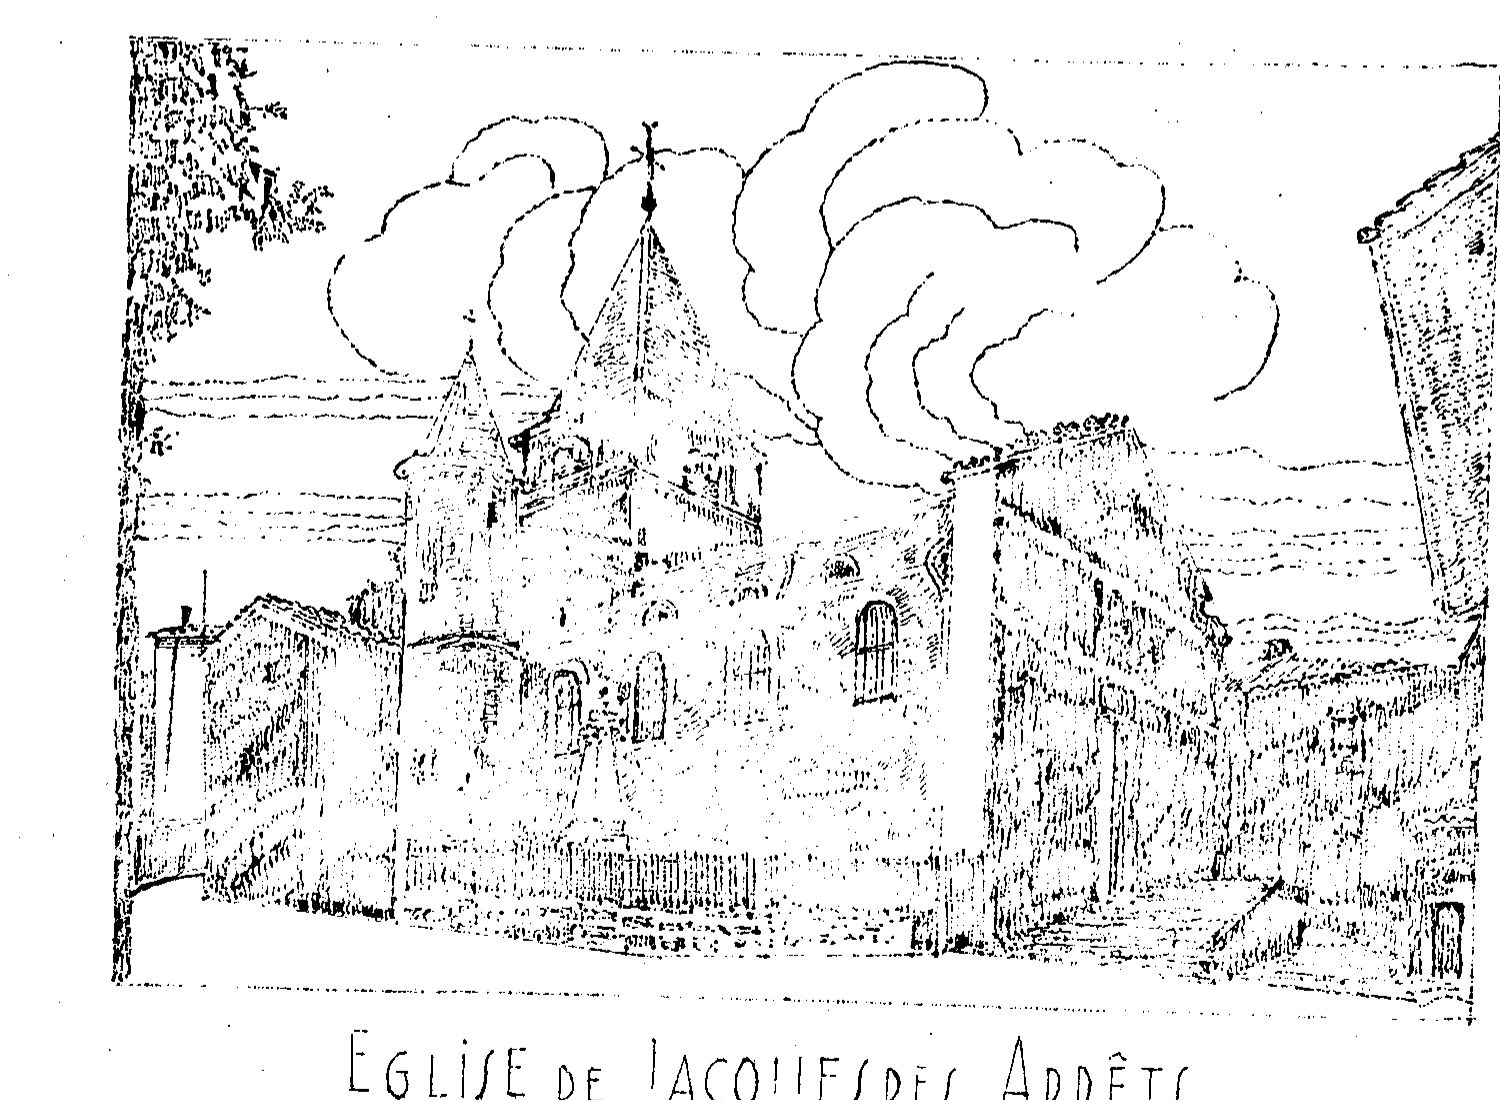
\includegraphics[width=0.70\textwidth]{Illustrations/illus-revolution-jacques-arrets.png}
\end{figure}
% --- Page imprimée 157 — vue 160 (suite)
te on était en dehors de tout danger.

Mais parmi ses fabriciens il y avait un traître. Celui-ci communiqua aux autorités révolutionnaires le plan qui venait de lui être détaillé. Il suffira de mettre un factionnaire dans la rue, près de la porte du puits ; un autre pénétrera dans la cure, impossible au curé d'échapper.

On saisit avec empressement l'occasion qui s'offrait de s'emparer d'un prêtre pour le livrer aux tribunaux révolutionnaires. Les gendarmes furent-ils chargés eux-mêmes du mandat d'amener ? ou bien les gardes nationaux qui avaient reçu le titre de "brigands" procédèrent-ils eux-mêmes à l'arrestation du pauvre prêtre ? Cette dernière hypothèse est fort probable car nous savons que la garde nationale de Beaujeu se donna plus d'une fois cette triste mission. Elle parcourait nos montagnes jetant partout l'effroi par ses arrestations arbitraires, par ses déprédations sans cesse renouvelées. Ses victimes, une fois livrées à la gendarmerie étaient conduites à Villefranche, puis à Lyon, pour entendre prononcer leur sentence et être exécutées.

Nous savons que Mr Donjon fut guillotiné et mourut en confessant la foi catholique. Mr Polloce, dans une note ajoute que tous ses persécuteurs moururent misérablement.

Les impies n'étaient pas satisfaits. Obligés de repasser à Ouroux pour se rendre à Beaujeu, ils résolurent de se venger de la réception peu sympathique qui leur avait été faite quelques heures auparavant dans le bourg. Ils entrèrent donc dans l'église, la dévastèrent complètement et brisèrent la chaire et les confessionnaux. Ils descendirent le grand crucifix qui selon l'usage du temps était placé sous l'arceau qui sépare le chœur de la nef, dressèrent un bûcher au haut du jardin de Mr Duligier qui est devenu la place actuelle, devant la maison de Chambru aubergiste et le brûlèrent en présence de Mr le curé de St-Jacques. Ils disaient à leur prisonnier en le raillant : "nous avons brûlé ton Bon Dieu". Ceci avait lieu en 1792.

Comment les nombreux tableaux et les statues des saints échappèrent-ils à ces actes de vandalisme ? Nous l'ignorons. L'attitude de la population ne leur permit-elle pas de tout anéantir ? Ou bien la
% --- Page imprimée 158 — vue 161 (suite)
présence du curé constitutionnel leur imposa-t-elle un reste de pudeur ? Le fait est que les tableaux et les statues furent conservés.

Ces objets sans valeur ne pouvaient, il est vrai, exciter beaucoup leur convoitise ; il n'en fut pas de même pour les objets précieux dont notre église était si bien fournie au commencement de la Grande Révolution. Il est difficile d'établir une liste complète de tout ce qui disparut à cette époque. Nous ne pouvons que mentionner les ornements achetés par Mr Guillin et qui furent pris par les autorités du district ou par les pillards eux-mêmes. Notre église possédait alors des chandeliers d'argent qui avaient coûté 1321 livres et un crucifix du même métal à la confection duquel on avait employé 366 livres de matière précieuse ; deux autres chandeliers d'argent ayant coûté 634 livres, un encensoir et sa navette, des burettes et leur plateau, le tout en argent et estimé 520 livres. Les calices et les ciboires subirent également le même sort puisque Mr Trouilloux fut obligé d'en acheter à son retour de l'exil.

Le décret de la Convention ordonnant aux municipalités d'avoir à livrer les cloches des paroisses pour fournir le bronze des canons à l'exception d'un timbre pour l'horloge, fut fidèlement exécuté à Ouroux. Nous avons vu que notre clocher en renfermait quatre à la mort de Mr Guillin. Le 5 Juin 1797 Mr Trouilloux donnait à un ouvrier 25 livres pour réparer la cloche que l'on avait laissée. Le clocher lui-même eut beaucoup à souffrir de l'injure du temps et des dégâts qui y furent commis ; comme pour l'église, le curé intrus négligea toute réparation.

La loi du 9 Novembre 1789 ne fut exécutée à Ouroux que longtemps après. Cette loi, on le sait, mettait à la disposition de la nation tous les biens ecclésiastiques, à la charge, pour elle, de pourvoir aux frais du culte et aux traitements des ministres. Toutefois celle du 12 juillet 1790 portait sursis à la vente des biens affectés à des fondations pieuses. Enfin la loi du 18 octobre 1790 et celle du 20 Décembre de la même année fixant à ½ arpent ou à 1/4 d'hectare la contenance du jardin affecté aux presbytères fut suivie de la loi du 19 Août 1792 qui prescrivait la vente des immeubles réels affectés aux fabriques des églises. On se mit donc en mesure de vendre le
% --- Page imprimée 159 — vue 162 (suite)
pré qui appartenait à la cure d'Ouroux et qui est situé entre le cimetière et la rivière. Une partie de ce pré avait été donnée à la cure pour acquitter les 5 messes fondées en 1707 par Jean Hugues et Jean Chrysostome Duligier à leur chapelle N.D. de Grés.

En conséquence le 5 thermidor an III (23 juillet 1795) le procureur syndic de Villefranche procéda à la mise en adjudication du demi-arpent, réservant le jardin attaché au presbytère. Les premières enchères furent fixées à la somme de 1125 livres ; aucun citoyen acquéreur ne se présenta. On fixa au 21 thermidor la vente définitive. Cette fois les acquéreurs ne faisaient pas défaut. L'acte de vente porte en effet qu'il fut allumé sept feux pendant lesquels les mises s'élevèrent à la somme de 10000 livres. Le citoyen Julien Chagny, propriétaire à Ouroux et fermier à Grosbois tenant la dernière mise, le pré lui fut adjugé.

Le 9 pluviôse an IV (29 janvier 1796) par acte reçu Mr Jandard, notaire à Monsols, Julien Chagny était remboursé des 10000 livres en assignats par Jean Lardet et Benoît Laplace qui servirent de prête-nom et restituèrent à la cure le bien injustement aliéné. Par qui fut fournie cette somme ? les registres de la fabrique ne donnent à ce sujet aucune indication.

Cette somme de 10000 livres nous paraît exorbitante. Mais il faut se rappeler l'énorme dépréciation des assignats à cette époque. Déjà pendant l'année 1792 ils avaient perdu 34,40 \% et 47 \% en janvier, février et mars. En 1793 ils perdirent encore pendant les mêmes mois 45 et 50 \%, en mai, juin, juillet 54,60 et 67 \%.

Enfin Ouroux comme châtiment de sa fidélité à la foi catholique, vit disparaître son ancien nom. La Convention, on le sait, avait résolu d'abolir tout ce qui rappelait l'ancien ordre de choses. Le 22 septembre 1792 commençait l'année républicaine avec son nouveau calendrier offrant à la place du nom des saints le nom des animaux, des instruments, des plantes, des minéraux. Les paroisses elles-mêmes qui le plus souvent avaient pris le titre du saint sous la protection duquel elles avaient été placées à l'origine, subirent la loi commune. Le nom de St-Antoine d'Ouroux dut disparaître pour faire place à celui de Valcivique, nom tiré de sa position dans la vallée.

% --- Page imprimée 160 — vue 163
"Ce jourd'hui 23 nivôse an II de la République une, indivisible, démocratique et impérissable, pardevant nous Louis Matray, maire de la commune de Valcivique cy-devant Ouroux" tel fut le premier titre où il est fait mention de ce nouveau nom.

Néanmoins, il était difficile de briser avec la tradition, de faire disparaître un nom connu de tous et le terme de Val-Civique n'est employé que fort rarement et dans les occasions où les pièces officielles devaient passer sous les yeux des autorités républicaines. Et même à Ouroux, il s'en trouvait qui aimaient à flatter leur amour-propre en se distinguant des simples mortels par une adhésion publiquement affichée aux nouvelles idées du jour. Louis Matray, dans les pièces qu'il a rédigées en offre souvent des preuves. Néanmoins, chose curieuse, le nom de Val-Civique n'est pas employé dans l'acte de vente du pré de la cure.

Dans la correspondance de la famille Duligier à cette époque, nous trouvons habituellement le terme de Val-Civique au lieu de celui d'Ouroux. Sa position lui en faisait, il est vrai, une sorte de loi. Il se demandait pour sa tante, ancienne religieuse visitandine à Mâcon, la pension que la loi avait accordée aux religieuses chassées de leur couvent. Il était naturel, dès lors, qu'il flattât les hommes du jour en entrant publiquement dans leurs vues. Je ne citerai que cette adresse qui nous apprend en même temps le changement du nom de St-Sorlin (Saône et Loire) : "À la citoyenne Duligier Testenoire, cy-devant religieuse visitandine de Mâcon à Rochevineuse cy-devant St-Sorlin, à la commune de Val-Civique district de Villefranche.

La Terreur ayant pris fin, Ouroux recouvra son ancien titre et de tous ces changements absurdes et impies, il en reste à peine le souvenir.

Mr Trouilloux ayant repris possession de sa paroisse, mit tout en œuvre pour réparer les désastres matériels et moraux qu'elle avait eu à subir. Rien d'intéressant comme l'étude de ses dépenses inscrites consciencieusement au jour le jour, nous le montrant luttant contre des difficultés de toutes sortes, n'ayant à sa disposition que des ressources précaires et insuffisantes.

% --- Page imprimée 161 — vue 164
C'est un bénitier en fer blanc qu'il doit payer 60 livres en assignats (1795), deux livres d'encens, 100 livres également en assignats. Et ainsi pour tout le reste. Point de recettes dans la fabrique, le culte, sans doute, ne pouvant s'exercer que très irrégulièrement à l'église malgré le décret du 21 février 1795 n'interdisant aucun culte qu'il n'était pas ostensible.

Ce n'est qu'en 1797 que tout rentra dans l'ordre au milieu de nous. Les dépenses et les recettes reprennent leur cours normal. Au mois de mai de cette même année on met aux enchères les places de l'église qui fournissent une somme de 516 livres, résultat considérable qu'on n'atteignit jamais les années suivantes. On comprend avec quel empressement religieux la population restée fidèle au milieu de si longues épreuves, reprit possession de son église profanée et tint à honneur de s'asseoir de nouveau sur ces bancs qui portaient encore la trace du vandalisme révolutionnaire.

Mais il est une dépense insignifiante en apparence que je ne saurais passer sous silence; elle nous permettra d'établir une date hypothétique il est vrai, mais importante dans l'étude qui nous occupe.

Nous trouvons inscrit au mois de mai 1795 une somme de 9 livres pour "souliers au conducteur de Mr le Curé". Comme toutes les autres dépenses, celle-ci est inscrite par Trompier qui avait interrompu ses études à la suite de la Constitution Civile du Clergé et qui devait néanmoins être prêtre un jour. Quel était donc ce conducteur?

On peut supposer que Mr Trouilloux, à son retour d'exil, continuant à se cacher, mais voulant néanmoins faire profiter de son ministère les diverses paroisses privées encore de leurs pasteurs, se faisait accompagner dans ses courses par un homme dévoué; la fabrique voulant témoigner à ce dernier combien elle comprenait son dévouement lui fit ce don qui nous paraît à cette heure, de minime importance mais qui n'en était pas moins précieux dans ces temps de misère.

Je m'arrêterai toutefois plus volontiers à cette autre supposition qui me paraît de beaucoup plus probable. Cet homme ne serait autre que le guide accordé à Mr Trouilloux à son entrée en France.

% --- Page imprimée 162 — vue 165
Il lui eut été difficile, pour ne pas dire impossible, de traverser seul la région qui nous sépare de la Suisse où il s'était réfugié.

A ce titre d'émigré il courait toujours risque d'être arrêté et il était prudent de s'adjoindre un compagnon de route connaissant les lieux, ayant des relations dans les contrées qu'il fallait traverser, prouvant, grâce à son titre d'étranger et un passeport en règle, voyager en toute sécurité. Mr Trouilloux, à son arrivée à Ouroux étant dénué de tout et ne voulant pas renvoyer son conducteur sans lui accorder une gratification, les fabriciens lui seraient venus en aide. La somme proprement dite fixée par le guide avait pu être payée en Suisse même par les comités organisés à l'étranger pour venir en aide aux malheureux prêtres forcés de quitter leur patrie.

Ainsi grâce à ce détail, l'époque du retour de Mr Trouilloux serait fixée ; ce serait au mois de mai de l'année 1795. Cette conclusion, nous l'avions déduite, mais sans preuves positives, des actes de catholicité. Notre hypothèse vient fortifier ce sentiment.

J'ai dit que le culte religieux fut rétabli complètement en 1797. Cette année-là, Mr Trouilloux acheta des vases sacrés plus dignes de la paroisse : calice, ciboire, encensoir, ostensoir. Il fit de plus donner une mission dans le but de tranquilliser les consciences et de permettre aux égarés de rentrer en grâce avec Dieu. Une croix fut plantée en souvenir de cette mission. On sait que ce fut là le moyen principal que l'autorité religieuse employa dans notre région pour mettre fin à tous les désordres, régler les questions d'intérêt qui furent si importantes à cette époque.

Et cependant si nous consultons l'histoire, nous voyons que l'année 1797 fut féconde en incidents de toute sorte. Un instant même, on crut rentrer dans une nouvelle Terreur. Au mois de Septembre les églises furent de nouveau fermées, le culte catholique défendu, un nouveau serment imposé aux prêtres : « Je jure haine à la royauté et à l'anarchie, attachement et fidélité à la République et à la Constitution de l'an III ». Ceux qui refusèrent de le prêter furent poursuivis comme en 1793. Un grand nombre furent déportés dans les déserts insalubres de Konamama ou de Sinnamary à Cayenne où ils moururent pour la plupart.

% --- Page imprimée 163 — vue 166
Il ne semble pas, néanmoins que Mr Trouilloux ait eu à souffrir pendant ce nouvel orage. Ouroux avait donné une première fois assez de preuve de son énergie pour qu'on n'essayât pas de jeter de nouveau le trouble dans la paroisse. Les premiers persécuteurs, du reste, avaient payé leur dette à la justice divine et ceux qui vivaient encore avaient appris à concentrer leur impiété et leur rage à la vue de ce culte qu'ils avaient cru anéantir et qui renaissait après huit ans de persécution.

Mr Trouilloux paraît être resté seul à Ouroux jusqu'au rétablissement de la paix religieuse par le Concordat. Lui seul en effet a signé les actes de l'état religieux pendant cette période. Nous n'avons que quelques rares signatures de Mr Odin pendant les années 1796 et 1797 ; nous ne le retrouvons plus jusqu'au 7 mai 1801. Il est vraisemblable qu'il fut nommé à ce moment curé de St-Nizier d'Azergues. Mais que fit-il pendant cet intervalle de 4 ou 5 ans qu'il a passé loin de notre paroisse ? Il fut probablement appelé par l'autorité supérieure ou même encore par ses confrères à porter le secours de son ministère à quelque paroisse dépourvue de prêtres ; peut-être aussi se dévoua-t-il à l'œuvre si importante des missions car ce n'était pas chose facile que de ramener une paroisse lancée dans la mauvaise voie, abandonnée depuis longtemps, scandalisée par ceux mêmes qui auraient dû la maintenir dans la vraie foi.

Mr Odin avait, pendant ces huit années de persécutions, acquis de l'expérience ; il reconnaissait toutes les misères des populations. Il avait, grâce à son dévouement, conquis dans nos montagnes une influence qu'il était naturel de faire servir à la réhabilitation de l'Église auprès des égarés. Il dut donc partir, évangélisant tantôt une paroisse, tantôt une autre, conservant néanmoins son titre de vicaire d'Ouroux que la Constitution Civile du Clergé n'avait pas été capable de lui enlever, jusqu'au jour où l'autorité fit de nouveau appel à son zèle pour diriger une paroisse importante comme l'était celle de St-Nizier d'Azergues.

Il vint attendre à Ouroux la décision qui allait être prise à son égard, et, c'est pendant les quelques jours qu'il demeura dans la paroisse qu'il put prêter de nouveau à son digne curé le secours de
% --- Page imprimée 164 — vue 167 (suite)
son ministère. Voilà, je le répète, l'explication la plus plausible que l'on peut donner de la longue absence de Mr Odin et de sa présence comme vicaire à Ouroux pendant le mois de mai de l'année 1801

Il partit donc à St-Nizier, emportant les regrets de la population toute entière. Les personnes pieuses qui l'avaient connu et qui avaient su apprécier la sagesse de sa direction ne l'oublièrent pas. On aimait, encore longtemps après, aller à St-Nizier pour le voir, lui demander des conseils ; il était heureux lui-même de retrouver ses anciens d'Ouroux. Les parents se faisaient même accompagner parfois de leurs enfants que Mr Odin avait baptisés pendant la tourmente révolutionnaire et c'était pour ce saint prêtre un bonheur de rappeler dans ses conversations les épreuves et les joies de ces temps malheureux mais si féconds en héroïques dévouements.

Mr Odin était né à Rozier-Côtes-d'Aurec, paroisse du canton de St Bonnet le Château, département de la Loire ;

Un mot sur les paroisses voisines.

Nous avons vu que Mr Odin évangélisa la plupart des paroisses de nos montagnes du Beaujolais. Il peut être intéressant de donner brièvement quelques détails sur la situation de ces paroisses pendant la Révolution. À cette heure, les souvenirs s'effacent vite et la génération qui grandit ne soupçonnera même pas quelles luttes ses ancêtres eurent à affronter pour conserver leur foi.

\begin{wrapfigure}{l}{0.40\textwidth}
    \vspace{-0.4\baselineskip}
    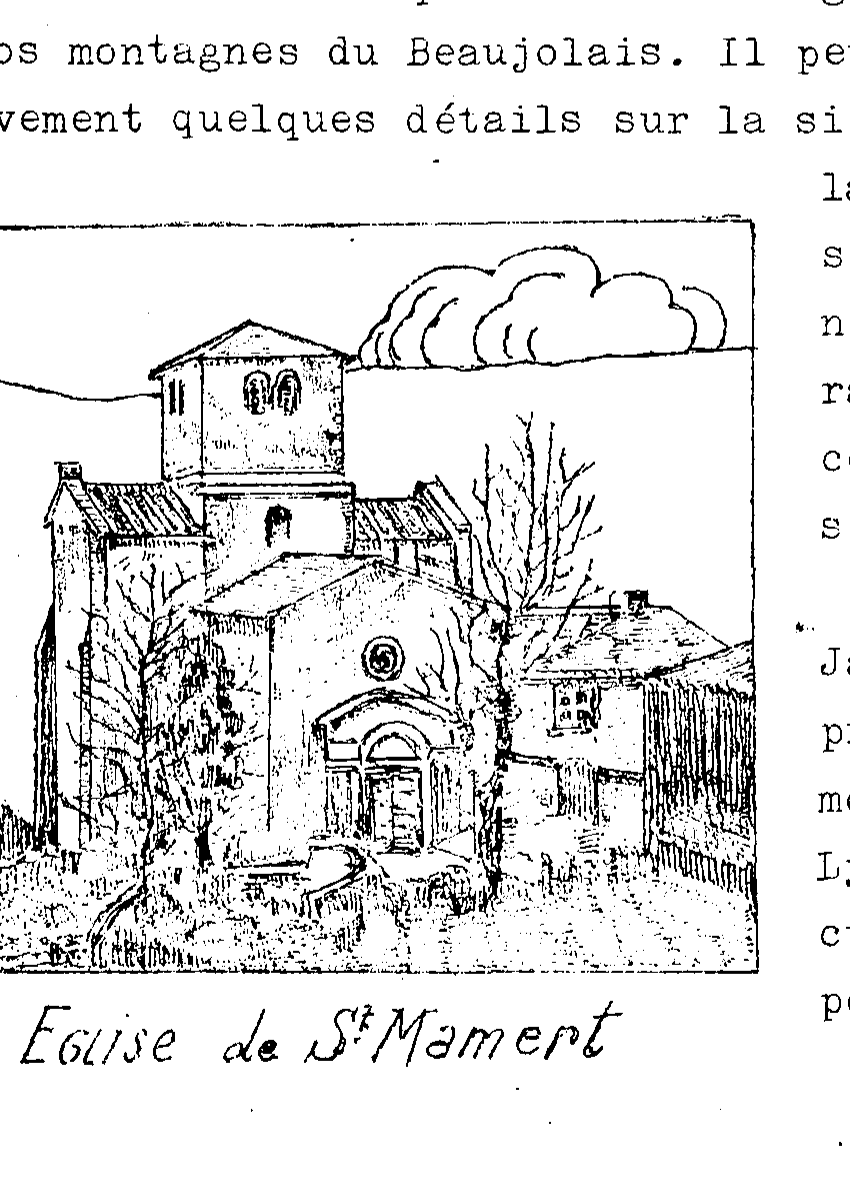
\includegraphics[width=0.36\textwidth]{Illustrations/illus-revolution-saint-mamert.png}
\end{wrapfigure}

Nous avons parlé plus haut de St Jacques des Arrêts. Le curé Donjon prêta serment, puis se rétracta et mourut en catholique, guillotiné à Lyon sur la place des Terreaux. Le curé intrus qui lui succéda s'appelait De Bardonenche.

Le curé constitutionnel de St 
% --- Page imprimée 165 — vue 168 (suite)
Mamert fut un nommé Picaud. Mr Odin fit la plupart des baptêmes dans les maisons particulières au fond des cachettes.

La paroisse de Cenves conserva pendant toute la tourmente son pasteur Mr Bouchacourt, qui demeura fidèle. L'esprit de foi de la population lui fournit des asiles sûrs, malgré les recherches dont il fut l'objet. Tout le monde sait que Mgr Daviau du Bois de Sauzay archevêque de Bordeaux fit une ordination de plusieurs prêtres dans un village situé dans la vallée, près du Vieux-Château. La chambre, dans laquelle eut lieu la cérémonie existe encore à cette heure.

St-Christophe-la-Montagne eut aussi son curé assermenté dont j'ignore le nom. Mr Canard né au hameau du Pasquier situé dans cette même paroisse, ayant été ordonné prêtre à Fribourg revint à St-Christophe et travailla avec un plein succès à la ramener à la foi catholique.

Le curé de Monsols ajouta le scandale au schisme dans lequel il n'avait pas craint de s'engager. Cette paroisse fut évangélisée après la Terreur par Mr Odin surnommé le petit Toine par opposition au grand Toine et dont il était probablement le parent.

Celui de Beaujeu, Gaudet, prêta serment, fut arrêté comme suspect et fusillé aux Brottaux. Il fit savoir à Mr Chuzeville, vicaire à Grandris alors en prison qu'il s'était rétracté en allant au supplice et qu'il avait pu bénéficier ainsi de l'absolution qu'un prêtre placé à une fenêtre de la place des Terreaux donnait à chaque condamné à sa sortie de prison. Tout le clergé séculier et régulier de Beaujeu prêta serment à l'exception de Mr de Chastié. Mr Odin, vicaire d'Ouroux contribua dans une large mesure au retour de la vraie foi de cette ville importante du Beaujolais. Il fut admirablement secondé par Mr Guérin curé d'Avenas et quelques autres qui trouvaient une hospitalité généreuse dans la famille Testenoire

Mr Guérin curé d'Avenas né à Belleroche mérite une mention spéciale. Arrêté à Poulle, au hameau de Longefaix par les brigands de St-Didier sur Beaujeu, le 11 Avril 1793, il fut conduit à Villefranche escorté par les gendarmes. Son passage à Beaujeu fut marqué par un incident dont le souvenir est toujours vivant et grâce auquel il
% --- Page imprimée 166 — vue 169 (suite)
a dû se conserver la vie. Un maître-maçon nommé Petit qui travaillait aux constructions que l'on élevait à ce moment à l'hôpital, revenait de prendre son repas lorsqu'il apprend le départ de Mr Guérin pour Villefranche. Furieux il monte sur son échafaud, prend son marteau et invite ses ouvriers à le suivre afin d'immoler au pied de l'arbre de la liberté ce prêtre réfractaire, l'ennemi de la patrie. Mr Guérin, attaché à la selle de l'un des chevaux des gendarmes et les menottes aux mains débouche devant l'église et le cimetière de Beaujeu. À ce moment Petit lève son marteau pour le frapper ; le malheureux tombe raide mort. Les médecins accourent, lui prodiguent leurs soins ; peine inutile, la justice de Dieu était bien satisfaite.

Ce confesseur de la foi eut pour compagnon de captivité Mr Chuzeville vicaire à Grandris, à l'époque du serment. Il est mort curé des Ardillats dans un âge avancé. Comme Mr Guérin il fut pris par la garde nationale de Beaujeu composée de 60 à 70 hommes, au bourg même de Poulle, dans un fenil où il s'était caché. Conduit à Villefranche, puis à Lyon où il retrouva son ami Mr Guérin, il fut condamné comme lui à être déporté sur le vaisseau à Rochefort. Là ils restèrent pendant deux ans et grâce à leur robuste constitution, ils purent résister aux terribles épreuves qui firent périr un si grand nombre de prêtres. À la chute de Robespierre ils furent mis en liberté et vinrent dans leurs anciennes paroisses relever les courages abattus, ramener les égarés et continuer un ministère qui ne cessa d'être fécond. Mr Guérin eut comme successeur comme curé intrus un nommé Gelin.

Ces quelques détails sur les localités voisines d'Ouroux et leur situation à cette époque néfaste nous feront remercier la divine Providence d'avoir épargné à notre paroisse les épreuves qu'elle permit à l'égard de tant d'autres. Rien de surprenant dans les défections sans nombre et les faiblesses dont ces populations se montrèrent coupables. Si Ouroux sut résister aux affronts du schisme, ce fut grâce aux efforts de Mr Odin qui contrebalança, par sa vigilance et ses conseils, l'action des prêtres constitutionnels.
